\documentclass[a4paper]{report}
\usepackage[utf8]{inputenc}
\usepackage[portuguese]{babel}
\usepackage{a4wide}
\usepackage{hyperref}
\hypersetup{pdftitle={Transformador Publico2NetLang},
pdfauthor={Joao Teixeira, Jose Filipe Ferreira, Miguel Solino},
colorlinks=true,
urlcolor=blue,
linkcolor=black}
\usepackage{subcaption}
\usepackage[cache=false]{minted}
\usepackage{listings}
\usepackage{booktabs}
\usepackage{multirow}
\usepackage{appendix}
\usepackage{tikz}
\usepackage{authblk}
\usepackage[parfill]{parskip}
\usetikzlibrary{positioning,automata,decorations.markings}

\begin{document}

\title{Transformador Publico2NetLang \\
\large TP1 - Exercício 4 - Grupo 7}
\author{Joao Teixeira (A85504) \and Jose Filipe Ferreira (A83683) \and Miguel
Solino (A86435)}
\date{\today}

\begin{center}
    \begin{minipage}{0.75\linewidth}
        \centering
        
\includegraphics[width=0.4\textwidth]{eng.jpeg}\par\vspace{1cm}
        \vspace{1.5cm}
        \href{https://www.uminho.pt/PT}
        {\color{black}{\scshape\LARGE Universidade do Minho}} \par
        \vspace{1cm}
        \href{https://www.di.uminho.pt/}
        {\color{black}{\scshape\Large Departamento de Informática}} \par
        \vspace{1.5cm}
        \maketitle
    \end{minipage}
\end{center}

\begin{abstract}
    \begin{center}
        O objetivo deste projeto é processar um ficheiro HTML para produzir um
        JSON organizado, utilizando \textit{FLex} para gerar um parser eficiente
        utilizando expressões regulares.
    \end{center}
\end{abstract}

\tableofcontents

\pagebreak

\chapter{Introdução}
Este projeto tem como objetivo o processamento de um ficheiro \textit{HTML}
contendo os comentários de uma notícia de forma a extrair todos os dados
relevantes e transformá-los num formato \textit{JSON}.

Para o processamento deste ficheiro foi escrito um filtro de texto utilizando 
o gerador \textit{FLex} e a linguagem de programação C.

Em primeiro lugar iremos analisar o problema, determinar que funcionalidades 
implementar e identificar os desafios que serão necessários ultrapassar
para implementar essas funcionalidades.

Em seguida iremos analisar a nossa solução, a estrutura do \textit{parser},
como foram escolhidos os subcontextos, que expressões regulares foram
escolhidas para os construir e a estrutura do projeto onde iremos falar
das estruturas de dados utilizadas.

Para concluir, iremos apresentar um pequeno manual de utilização do programa.

\chapter{Problema}

O programa tem que cumprir os seguintes requisitos:
\begin{itemize}
    \item Converter o ficheiro de input para \textit{UTF-8};
    \item Identificar no ficheiro de \textit{input} os diversos comentários;
    \item Separar os diferentes elementos dos comentários;
    \item Garantir que as respostas a um comentário são guardadas de forma
        aninhada;
    \item Contar o número de respostas a cada comentário;
\end{itemize}

O ficheiro de \textit{input} apresentou vários problemas que precisa de ser
tratados para conseguir cumprir os requisitos propostos.

O primeiro sendo a codificação do ficheiro que está em \textit{latin1} e é
preciso converter para \textit{UTF-8} de forma a que o output do programa não
apareça com caracteres ilegíveis.

O segundo foi o facto de alguns dos comentários apresentados conterem mais do que
uma linha, invalidando assim o \textit{JSON} de output se não forem tratados.

\chapter{Solução}

\section{Contextos de Processamento}

Para processar o ficheiro com os comentários foram implementados 7 subcontextos:
\textit{DEFAULT}, \textit{THREAD}, \textit{CONTENT} (identificado a amarelo),
\textit{ID} (identificado a vermelho), \textit{USER} (identificado a azul),
\textit{DATE} (identificado a verde) e \textit{REPLY} (identificado a roxo).

\begin{figure}[H]
    \centering
    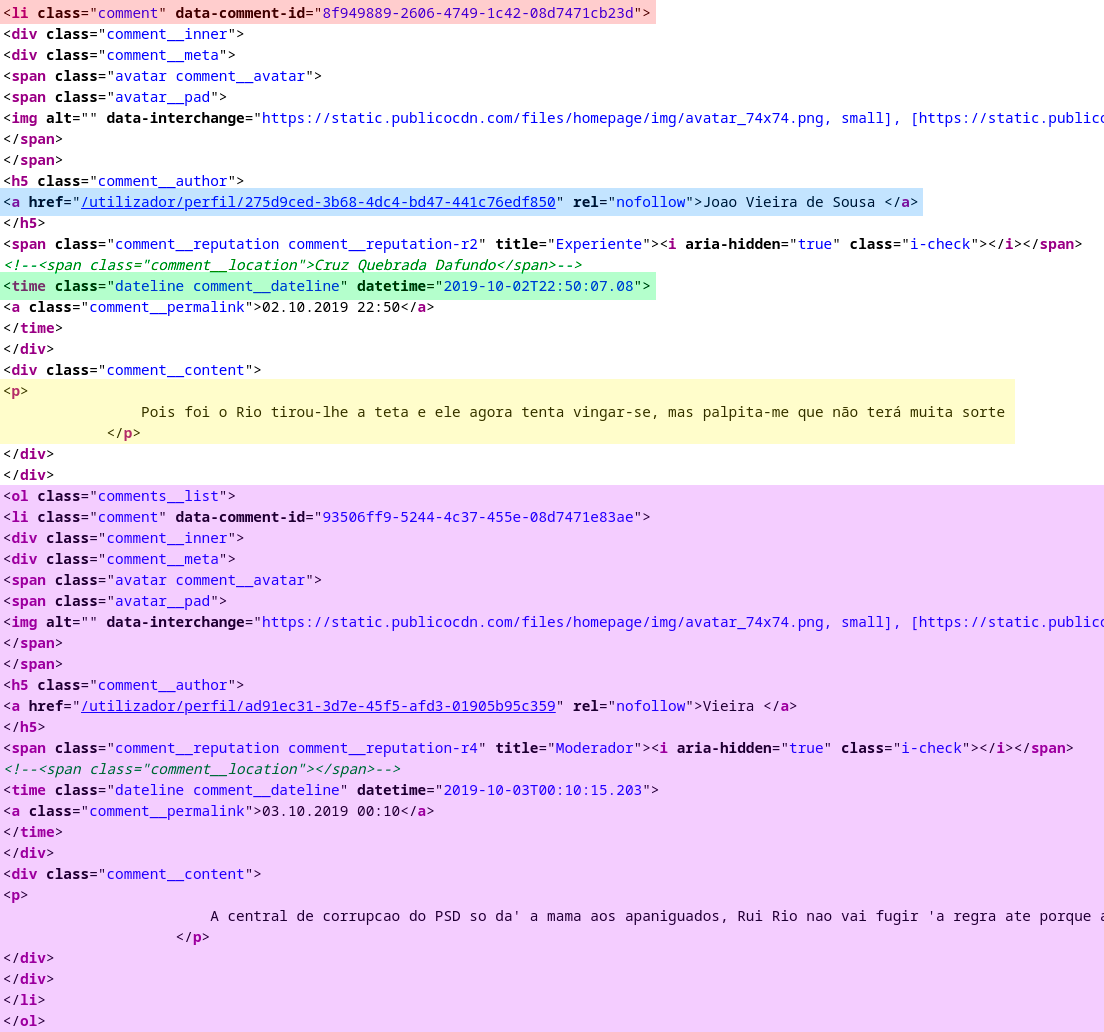
\includegraphics[width=0.88\textwidth]{states.png}
    \caption{Comentário e respostas com os contextos identificados}
\end{figure}

\subsection{DEFAULT}

Toda a zona correspondente ao contexto DEFAULT é ignorada, pois é a zona
que contem a informação irrelevante ao programa.

\subsection{THREAD}

No THREAD é onde se encontra a informação relevante sobre os comentários,
e onde estão contidos todos os subcontextos descritos abaixo.

\begin{figure}[H]
    %Requires:
%\usepackage{tikz}
%\usetikzlibrary{positioning,automata,decorations.markings}
\begin{tikzpicture}[font=\ttfamily,auto]
    \node[state,initial,accepting,text width=15mm,align=center] (thread) {THREAD};
    \node[state,text width=15mm,align=center] (id) [below=4.5cm of thread] {ID};
    \node[state,text width=15mm,align=center] (content) [above=4.5cm of thread] {CONTENT};
    \node[state,text width=15mm,align=center] (date) [right=5cm of thread] {DATE};
    \node[state,text width=15mm,align=center] (reply)  [left=5cm of thread] {REPLY};
    \path[thick,->]
    (thread)     edge [bend left=52] node [align=center] {\char`<p\char`>[ \char`\\r\char`\\n]*} (content)
                 edge [loop below] node {\char`<li class="comment\char`"} ()
                 edge [bend left=52] node {data-comment-id=} (id)
                 edge [bend left=12] node {datetime=\char`"} (date)
                 edge [bend left=12] node {\char`<ol class[\char`^\char`>]*\char`>\char`\\r\char`\\n} (reply)

    (content)    edge [bend left=52] node {\char`\\r\char`\\n *char`<char`/p\char`>\char`\\r\char`\\n} (thread)

    (id)         edge [bend left=52] node {\char`>} (thread)

    (date)       edge [bend left=12] node {\char`>\char`\\r\char`\\n} (thread)

    (reply)      edge [bend left=12] node {\char`<li class="comment\char`"} (thread)

    ;
\end{tikzpicture}


    \caption{Maquina de Estados do Parser}\label{fig:parser_state_machine}
\end{figure}

Na Figura \ref{fig:parser_state_machine} é descrito como as mudanças de
estados são efetuadas, e que expressões regulares as causam.
\pagebreak

\subsection{CONTENT}

Neste contexto é onde o conteúdo de cada resposta é tratado e formatado,
removendo espaços repetidos e escapando os caracteres \textit{'\textbackslash n'},
de forma a assegurar que o output do programa é válido.

\subsection{ID}

Aqui é onde é identificado o ID de cada resposta, ignorando todo o resto
presente neste contexto.

\subsection{USER}

À semelhança do contexto acima descrito, o USER é onde são identificados
os detalhes do utilizador criador do respetivo comentário.

\subsection{DATE}

No contexto DATE é feito o processamento tanto da data do comentário como
a \textit{timestamp} do mesmo.

\subsection{REPLY}

No contexto REPLY estamos dentro das respostas de um comentário. Aqui,
como o processamento é recursivo, voltamos a ter os contextos acima descritos,
pois respostas são comentários normais.

\section{Arquitetura do Projeto}

Graças à simplicidade do projeto, foi-nos possível resolver o problema num
só módulo não comprometendo a legibilidade da solução. Neste módulo é tratado
o input, selecionada a informação relevante presente e formatada para ir de
encontro ao formato pretendido.

Quanto a estruturas de dados, apenas mantemos em memória uma \textit{stack}
de contadores, para ser possível armazenar o número de respostas de um
comentário, respeitando a recursividade do processamento no campo das respostas.
Para a restante informação não nos foi necessário armazenar nada em memória,
dando \textit{flush} desta mal é processada.

\chapter{Manual de Utilização}

Este programa é de utilização simples, recebendo como argumento o ficheiro
HTML a ser processado, podendo ser chamado desta forma: 
\verb!./html2json path_to_input_file!.

Depois de processado, o JSON resultante irá ser retornado pelo \textit{stdout}.
Como o JSON não é formatado de uma forma muito legível o programa pode ser
encadeado com ferramentas processamento de JSON como, por exemplo, o \textit{jq},
para facilitar a leitura do mesmo. Isto pode ser feito com o comando exemplo
\verb!./html2json path_to_input_file | jq!. O resultado da formatação deste
será mais uma vez retornado pelo \textit{stdout}.

\chapter{Conclusão}

Para concluir, fazemos um balanço bastante positivo do projeto, conseguindo
atingir todos os requisitos definidos. A utilização de expressões regulares
para tratamento de strings mostrou ser algo extremamente poderoso, permitindo
simplificar tarefas que de outra forma seriam muito mais trabalhosas e demoradas.

Como trabalho futuro, gostaríamos de trabalhar mais a formatação do output
para facilitar a leitura do mesmo.

\appendix

\chapter{FLex}

\lstinputlisting[basicstyle=\scriptsize\ttfamily]
{flex.l}

\end{document}
